\newpage

\section{The TGG transformation protocol}

\genHeader

If you worked through Part IV of the handbook, you'll remember that we introduced \emph{bidirectional model transformations} via Triple Graph Grammars
(TGGs). These take an instance input model and apply a series of rules to generate a transformed output model and correspondence (or link) metamodel.
Together, these three files form the transformation's output \emph{graph triple}. You might also remember that we introduced an integrator in
Section 6, a visualizing tool that can help you trace a transformation via the correspondence model. 

While the integrator's display structure is based on the entire graph triple, its purpose is to interpret the key parts of the transformation's co-generated
\texttt{protocol} file, the detailed listing of every executed action. As you can imagine, examining this file directly provides much more detail than the
integrator alone. While both list the current step, element, rule candidates, and their results, the protocol includes properties of each step such as the
current element's full name, a listing of the created and/or translated elements, the reasons for a rule's success for failure, and other information.

To explain, let's revisit the running example as it was in Part IV, Section 7, where a fourth partition and card were added to a forward
transformation only able to handle three partitions. Let's start by reviewing the integrator as shown in Fig.~\ref{eclipse:integratorFWD}.

\begin{figure}[htbp]
\begin{center} 
  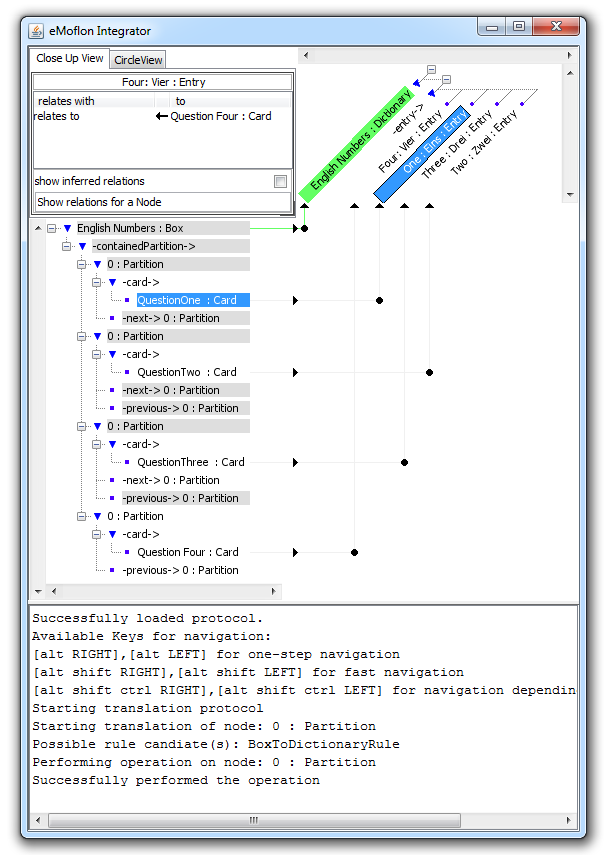
\includegraphics[width=0.8\textwidth]{eclipse_successBoxToDictionaryIntegrator}
  \caption{Integrator view of successful \texttt{BoxToDictionaryRule}}  
  \label{eclipse:integratorFWD}
\end{center}
\end{figure}

It begins the process by trying to translate the first node in the box, \texttt{part\-it\-ion\-0}. It checks for and applies the only valid rule, where each
navigation step shows the operation being executed in the display window. The final message tells us the rule was successful! Remember,
\texttt{BoxToDictionaryRule}\footnote{Refer to Part IV, Section 4, Fig. 28 (Visual) and Fig. 37 (Textual)} creates the primary container elements, \texttt{Box}
and \texttt{Dictionary}, and translates up to three connected \texttt{partitions}.

\newpage

Now let's see the equivalent transformation in the protocol file as depicted in Fig.~\ref{eclipse:protocolFWD}.

\vspace{0.5cm}

\begin{figure}[htbp]
\begin{center} 
  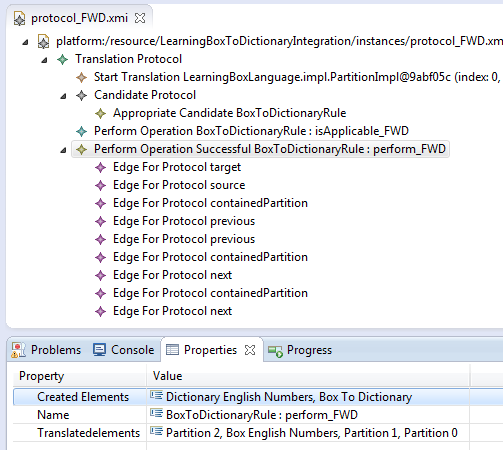
\includegraphics[width=0.9\textwidth]{eclipse_successBoxToDictionaryProtocol}
  \caption{Protocol file showing successful \texttt{BoxToDictionaryRule}}  
  \label{eclipse:protocolFWD}
\end{center}
\end{figure}

Again, the translation starts with the zero node (identified by its \texttt{index}) and finds a valid rule. It performs the rule, and lists its final result.
More information can be found however by double-clicking the success node, where the \texttt{Properties} window lists every element that was created and
translated. Finally expanding this successful node, we can then see further details about every edge that needed to be handled which in turn include details
such as their \texttt{name}, \texttt{Source}, and \texttt{Target} elements.

Let's skip ahead to something more interesting. Let's examine the place where the transformation starts trying to handle the erroneous fourth partition
(Fig.~\ref{eclipse:fourthPartition}).

\newpage

\begin{figure}[htbp]
\begin{center} 
  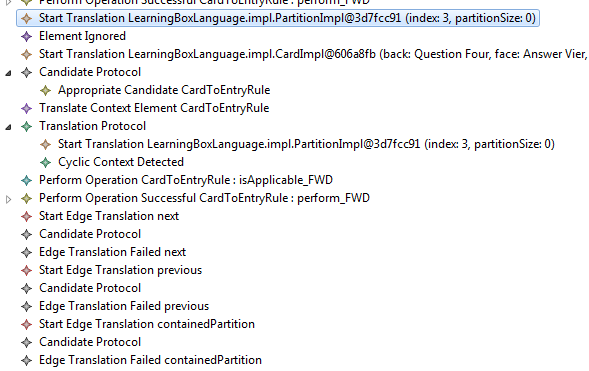
\includegraphics[width=\textwidth]{eclipse_fourthPartitionProtocol}
  \caption{Examining how the transformation succeeded}  
  \label{eclipse:fourthPartition}
\end{center}
\end{figure}

If you ran the integrator up to this point and finished the transformation, all you would see are indications that something has gone wrong -- the primary
window will highlight problematic elements in yellow, failed ones in red, and the message window below will list each step attempted but offer no
information. Examining the protocol however, we can see that the transformation isn't able to find any rule that can handle \texttt{partition3} (as indicated by
the lack of a `Candidate Protocol' beneath `Start Translation'). It's designed to follow an optimistic approach however, so the translation chooses to
simply ignore the element and try to translate its containing card first.

Sure enough, \texttt{CardToEntryRule}\footnote{Refer to Part IV, Section 4, Fig. 34 (Visual) and Fig. 41 (Textual)} is valid for \texttt{Question Four}, but
this rule's protocol requires it to try and establish the context partition. Once again, it tries to find a rule for \texttt{partition3}. At this point, the
transformation realizes it's doing the same thing over again (cyclic context detected) and chooses to ignore the partition a final time and proceeds to finish
the rule, successfully creating \texttt{Entry Four: Vier}. Finally, it tries to establish the edges connected to the failed partition with no luck.
